% ______________________________________________________________________________
%
%     1DV607 Object-oriented Analysis and Design 
%   Workshop 1 --- "Domain Modeling"
%
%   Author:  Jonas Sjöberg
%            Linnaeus University
%            js224eh@student.lnu.se
%            github.com/jonasjberg
%            www.jonasjberg.com
%
%  License:  Creative Commons Attribution 4.0 International (CC BY 4.0)
%            <http://creativecommons.org/licenses/by/4.0/legalcode>
%            See LICENSE.md for additional licensing information.
% ______________________________________________________________________________


\documentclass[11pt,a4paper]{article}


\usepackage[utf8]{inputenc}
\inputencoding{utf8}
\usepackage[swedish,english]{babel}
\usepackage[swedish]{isodate}
\usepackage[T1]{fontenc}

\usepackage{lmodern}
\usepackage{fullpage}

\usepackage{csquotes}
\usepackage[natbib=true,
            style=ieee,
            backend=biber]{biblatex}
\addbibresource{refs.bib}

\usepackage[binary-units=true]{siunitx}
\usepackage{float}
\usepackage{textcomp}
\usepackage{url}
\usepackage{graphicx}
%\usepackage{amssymb}
%\usepackage{amsmath}
\usepackage{amsfonts}
\usepackage{graphicx}
%\usepackage{microtype}


\usepackage[pdfusetitle,
            bookmarks=true,
            bookmarksnumbered=true,
            bookmarksopen=false,
            breaklinks=false,
            pdfborder={0 0 0},
            backref=false,
            colorlinks=false,
            hidelinks]{hyperref}

\usepackage{minted}
\usemintedstyle{bw}

\usepackage{verbatim}
\usepackage{fancyvrb}
\usepackage{listings}

% Used to remove numbering of some sections.
% \renewcommand*\thesection{\arabic{section}}

\renewcommand\listingscaption{Listing}
\renewcommand\listoflistingscaption{List of listings}

\usepackage{booktabs}
\usepackage{longtable}

\usepackage{pdfpages}


\title{\textsc{1DV607}                              \\
       Object-oriented Analysis and Design with UML \\
       Workshop 1                                   \\
       Domain Modeling               

\author{
  Jonas Sjöberg                          \\
  860224-xxxx                            \\
  Linnaeus University                    \\
  \texttt{js224eh@student.lnu.se}        \\
  \texttt{https://github.com/jonasjberg} \\
  \texttt{http://www.jonasjberg.com}
}

% \setcounter{section}{-1}
\date{}

\begin{document}
  \maketitle

  \begin{center}
    \begin{tabular}{l r}
      Written during:      & \isodate\printdate{2017-08-31} -- \isodate\printdate{2017-09-06} \\
      Teacher responsible: & Tobias Ohlsson
    \end{tabular}
  \end{center}

  \begin{abstract}
    The first workshop assignment in the course \emph{1DV607 -- Object-oriented
    Design and Analysis with UML} at Linnaeus University during the autumn term
    of 2017.  This workshop primarily covers initial domain modeling for some
    set of given fictional requirements, problem description and other
    background information provided by a simulated customer.
  \end{abstract}

  \clearpage
  %\hypersetup{linkcolor=black}
  \setcounter{tocdepth}{3}
  \tableofcontents

  \bigskip

  %\listoffigures
  %\listoftables
  %\listoflistings


  % ______________________________________________________________________________
%
%   1DV607 Objectorienterad Analysis och Design med UML
%   Workshop 1 --- "Domain Modeling"
%
%  Author:  Jonas Sjöberg
%           Linnaeus University
%           js224eh@student.lnu.se
%           https://github.com/jonasjberg
%
% License:  Creative Commons Attribution 4.0 International (CC BY 4.0)
%           <http://creativecommons.org/licenses/by/4.0/legalcode>
%           See LICENSE.md for additional licensing information.
% ______________________________________________________________________________


% ______________________________________________________________________________
\section{Problem Description}
%
% TODO: ..
%
The problem description \cite{1dv607:workshop1-instructions} is stated as
follows:

\begin{quote}
The yacht club ``The jolly pirate'' has started to get problems. The club has
grown to such an extent that the members have a hard time keeping track of all
meetings, and other important dates such as the club's various competitions. It
is also difficult for a member to change information in the membership
registry, for example change address or reporting that they have a newly
purchased boat. The result of this is that members sometimes are without a
reserved berth, when it became time for launch towards the spring.

The reservation of berths is operated by the club secretary and he goes through
all members’ boats and book their berth in the spring. This is a very ``tricky''
work, members owning several boats would love to have them as close together as
possible, while they want their ``usual'' place. Much fuss and mess usually
follow the announcement of this year’s places, and sometimes even ``private''
exchanges between members occurs, which strongly opposed by the municipality
for safety reasons.

The biggest problem, however, has the club’s treasurer, it is quite impossible
for the treasurer to manage all subscriptions manually via receipts that
members come in with when they paid their fees. The fee consists of a fixed
part and a variable part, where the variable component is dependent on the
number and the size of the boats. Several members probably slips through each
year without paying a fee, the result of wich is that the club will soon go
bankrupt.


\section{Actors}
\subsection{Primary Actors}
\begin{description}
  \item[Secretary]
  Wants to book berths for members in a fair and effective manner. Wants to
  minimize ``whining'' when advertising of berts and avoid that private
  exchanges occurs. Would also be able to manage the club’s calendar where
  important events and meetings are advertised.
  
  \item[Treasurer]
  Wants to manage member payments in an efficient manner. It is also important
  that the Treasurer has access to history in the payments for accounting
  purposes.

  \item[Member]
  A person who is a member of the boat club, probably has one or more boats
  registered and want a good berth for these. Want to manage their membership
  data, including boats, as well as to have a smooth overview of their
  payments.  Would also like to be able to participate in various boat club
  meetings and social activities.
\end{description}

\subsection{Offstage Actors}
\begin{description}
  \item[Municipality]
  Have an interest in knowing what boat owners have what berth. This is
  important in te event of for example example accidents, thefts or similar.
  
  \item[The tax authority]
  Have an interest in that the current regulations regarding the taxation of
  income associations are followed.
\end{description}


\section{Use Cases}
\subsection{Primary Actors}
\subsubsection{Secretary}\label{secretary}
Wants to book berths for members in a fair and effective manner. Wants
to minimize ``whining'' when advertising of berts and avoid that private
exchanges occurs. Would also be able to manage the club's calendar where
important events and meetings are advertised.

\subsubsection{Treasurer}\label{treasurer}

Wants to manage member payments in an efficient manner. It is also
important that the Treasurer has access to history in the payments for
accounting purposes.

\subsubsection{Member}\label{member}

A person who is a member of the boat club, probably has one or more
boats registered and want a good berth for these. Want to manage their
membership data, including boats, as well as to have a smooth overview
of their payments. Would also like to be able to participate in various
boat club meetings and social activities.

\subsection{Supporting Actors}\label{supporting-actors}

\subsubsection{Third-party systems for credit card
payment}\label{third-party-systems-for-credit-card-payment}

A service used to handle payment via credit card. Receives a transaction
ID and a sum, will respond with a positive or negative result.

\subsubsection{Third-party systems for Direct
Payment}\label{third-party-systems-for-direct-payment}

A service used to manage the direct payment online banking. Receives a
transaction ID and a sum, will respond with a positive or negative
result. In case of positive results money is deducted from the payer's
account 00:00 o'clock the next day, and the transaction may be rescinded
by the payer prior to tis alternatively, there is not enough money in
the account.

\subsubsection{Third party systems for SMS
payment}\label{third-party-systems-for-sms-payment}

A service for payment via SMS. A special message with the transaction id
is sent by the payer. This transaction id is provided by the service and
includes a checksum so that typing errors are minimized. The payment
will be deducted from the payer's phone bill.

\subsection{Offstage Actors}\label{offstage-actors}

\subsubsection{Municipality}\label{municipality}

Have an interest in knowing what boat owners have what berth. This is
important in te event of for example example accidents, thefts or
similar.

\subsubsection{The tax authority}\label{the-tax-authority}

Have an interest in that the current regulations regarding the taxation
of income associations are followed.

\subsection{Use Cases}\label{use-cases}

\subsection{1 Authenticate}\label{authenticate}

A person wants to be authenticated as a role. The person is
authenticated and assigned a role.

Precondition: The person is not already assigned a user role.

\subsubsection{Main scenario}\label{main-scenario}

\begin{enumerate}
\tightlist
\item
  The person wants to be authenticated.
\item
  The system asks for log in information.
\item
  The person supplies a user name and password
\item
  The system controls the username and password and authenticates the
  person as a user role (Member, Treasurer, Secretary) in the system,
  the assigned user role is presented.
\end{enumerate}

\subsubsection{Secondary Scenarios}\label{secondary-scenarios}

\paragraph{2.1 The combination of user name and password is
wrong}\label{the-combination-of-user-name-and-password-is-wrong}

\begin{enumerate}
\tightlist
\item
  The system presents an error message and asks for log in information
  again.
\item
  Go to step 3 in main scenario.
\end{enumerate}

\subsection{2 Pay Membership Fee}\label{pay-membership-fee}

A member wants to pay their dues. The fee and payment options are
presented and Member proceeds with payment. The payment is recorded and
its status is updated, a receipt is presented.

Primary Actor: User

\subsubsection{Main Scenario}\label{main-scenario-1}

\begin{enumerate}
\tightlist
\item
  The member wants to pay their dues.
\item
  The system presents the calculation of membership and a total amount
  due.
\item
  The member chooses to pay via credit card.
\item
  The system transmits a transaction id and a total to third-party
  system for Credit Card Payment.
\item
  Third Party Credit Card Payments System for process the transaction
  and reply with a positive result.
\item
  The system updates the Member's pay status to paid and presents a
  receipt of the transaction.
\end{enumerate}

\subsubsection{Secondary Scenarios}\label{secondary-scenarios-1}

\paragraph{3.1 The member chooses to pay via
invoice}\label{the-member-chooses-to-pay-via-invoice}

\begin{enumerate}
\tightlist
\item
  The system presents an invoice for printing with a unique invoice id,
  boat club account number and amount due. The amount due is the total
  membership fee plus an administrative service charge of currently 45
  swedish crowns.
\item
  The user confirms the invoice.
\item
  The system updates the member's payment status to invoiced and
  presents that the payment status changed.
\end{enumerate}

\paragraph{3.2 The member chooses to pay via SMS
payment}\label{the-member-chooses-to-pay-via-sms-payment}

\begin{enumerate}
\tightlist
\item
  The system contacts the Third Party System for SMS payment and enclose
  the sum total of the transaction.
\item
  The third-party systems for SMS payment replies with the SMS message
  to be sent to process the payment.
\item
  The system updates member's payment status to waiting. SMS message to
  be sent is presented.
\end{enumerate}

\paragraph{3.3 The member chooses to pay via third party systems for
Direct
Payment}\label{the-member-chooses-to-pay-via-third-party-systems-for-direct-payment}

\begin{enumerate}
\tightlist
\item
  The system transmits a transaction id and a total to third-party
  systems for Direct Payment.
\item
  Third Party System for Direct Payment process the payment and reply
  with a positive result.
\item
  The System updates the Member's pay status to paid and presents a
  receipt of the transaction.
\end{enumerate}

\subsection{3 View Member Profile
Information}\label{view-member-profile-information}

A member wants to view their member data. Membership details are
presented including registreade boats booked berths and payment history.

\subsection{4 Register Boat}\label{register-boat}

A member wants to register a new boat and the boat's data. The boat is
registered, the membership fee is updated and a confirmation appears.

\subsubsection{Main Scenario}\label{main-scenario-2}

\begin{enumerate}
\tightlist
\item
  A member wants to register a new boat.
\item
  The system asks for Boat Details.
\item
  The member input the boat's size and type (sailboat, motorsailer,
  powerboat, kayak/canoe, other) and an optional image of the boat.
\item
  The system presents the information for the boat to be registered,
  including cost of berth.
\item
  The member confirms the correct information.
\item
  The System registers the boat and assigns a berth using the current
  rules for berth assigment, updates the membership fee and presents a
  confirmation.
\end{enumerate}

\subsubsection{Secondary Scenarios}\label{secondary-scenarios-2}

\paragraph{\texorpdfstring{6.1 The boat is registered during the
``offseason'' (October 1 to December
31)}{6.1 The boat is registered during the offseason (October 1 to December 31)}}\label{the-boat-is-registered-during-the-offseason-october-1-to-december-31}

\begin{enumerate}
\tightlist
\item
  System assigns no berth and the membership fee for the current year is
  unchanged.
\end{enumerate}

\paragraph{6.2 The boat is registered in pre-season (January 1 to April
1) when no berth assignment has been made
yet.}\label{the-boat-is-registered-in-pre-season-january-1-to-april-1-when-no-berth-assignment-has-been-made-yet.}

\begin{enumerate}
\tightlist
\item
  System assigns no berth. This is done by the Secretary before the
  start of the season.
\end{enumerate}

\subsection{5 Remove a Boat}\label{remove-a-boat}

A Member To remove one of their registered boats. The boat is removed
and a confirmation appears.

\subsection{6 Change a boat.}\label{change-a-boat.}

A Member wants to change a boat's data. The boat's data is updated and a
confirmation appears.

\subsection{7 Send Payment Reminder}\label{send-payment-reminder}

The treasurer lists and send a reminder to those members who have not
paid enough dues for a calendar year.

\subsubsection{Main Scenario}\label{main-scenario-3}

\begin{enumerate}
\tightlist
\item
  The treasurer wants to send a reminder to those members who have not
  paid enough dues for a previous year and indicates the year
  considered.
\item
  The system lists the members who have a debt to the boat club during
  the year.
\item
  The treasurer choose to print an invoice for each member (see 2.3.1)
  in the invoice also includes a reminder fee of 25\% per year behind
  schedule.
\item
  The system prints an invoice per member and records that the member
  received a payment reminder.
\end{enumerate}

\subsection{8 Assign Berths}\label{assign-berths}

The Secretary wants to assign this season berths. The system assign and
book berths in accordance with applicable rules and update member
information.

\subsubsection{Main Scenario}\label{main-scenario-4}

\begin{enumerate}
\tightlist
\item
  The Secretary wants to book this season berths.
\item
  The system presents a proposal on the allocation under the current
  rules, the available berths and the previous year's allocation.
\item
  The Secretary approves the proposal.
\item
  The system assigns moorings for members' boats according to the
  proposal.
\end{enumerate}

\subsection{9 List Berths}\label{list-berths}

The secretary chooses to list all berths. A list of unbooked and booked
berths with information about the boat and member is presented.

\subsection{10 Manage Calendar Events}\label{manage-calendar-events}

The Secretary wants to add, delete or change a calendar event. Boat club
calendar is updated.

\subsection{11 List Calendar Events}\label{list-calendar-events}

A Member wish to list calendar events in a certain time interval. A list
of calendar events are presented with a short title and start date.

\subsection{12 View Calendar Events}\label{view-calendar-events}

Member to view all details for a particular calendar event. Calendar
event is presented including start and end dates.

\subsection{13 Update Payment Status}\label{update-payment-status}

The Treasurer would like to update the status of payments. The system
will contact third party services and check the status of payments and
update these.

\subsection{14 Update Invoice Status}\label{update-invoice-status}

The Treasurer wants to change a Member's payment status to paid. The
system updates the Member's payment status to paid.



\end{quote}


  % ______________________________________________________________________________
%
%   1DV607 Objectorienterad Analysis och Design med UML
%   Workshop 1 --- "Domain Modeling"
%
%  Author:  Jonas Sjöberg
%           Linnaeus University
%           js224eh@student.lnu.se
%           https://github.com/jonasjberg
%
% License:  Creative Commons Attribution 4.0 International (CC BY 4.0)
%           <http://creativecommons.org/licenses/by/4.0/legalcode>
%           See LICENSE.md for additional licensing information.
% ______________________________________________________________________________


% ______________________________________________________________________________
\section{Analysis}
The analysis is based on the given problem description\ref{probdesc}.
All work has been done by Jonas Sjöberg, without collaborators.


\subsection{Analysis of Requirements for Grade 2}
This analysis delimits the domain model to the following requirements:

\begin{itemize}
  \item \ref{usecase1} Authenticate
  \item \ref{usecase4} Register Boat
  \item \ref{usecase5} Remove Boat
  \item \ref{usecase6} Change Boat
  \item \ref{usecase8} Assign Berths
  \item \ref{usecase10} Manage Calendar Event
  \item \ref{usecase11} List Calendar Events
  \item \ref{usecase12} Show Calendar Event
\end{itemize}


\subsubsection{Domain Model for Grade 2}
\begin{figure}[htbp]
  \centering
  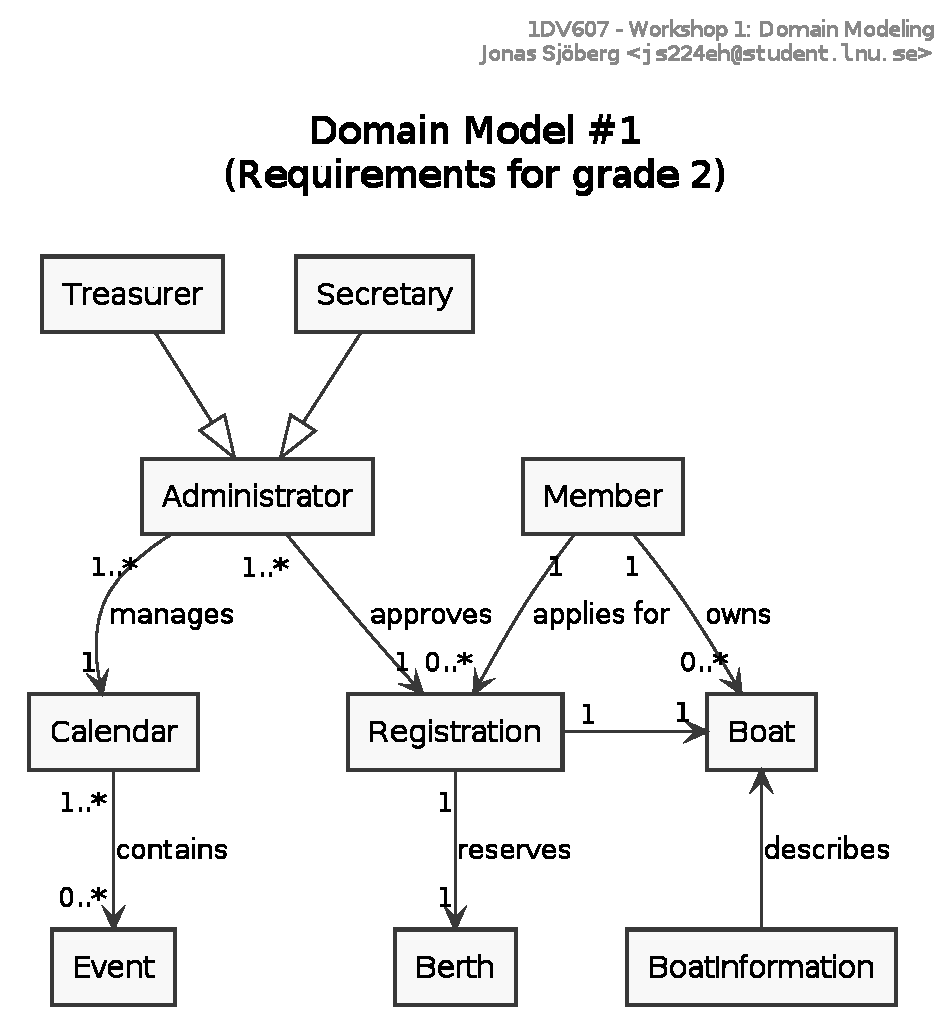
\includegraphics[width=\linewidth]{uml/domain-model_1.eps}
  \caption{UML Domain Model for Grade 2}
  \label{fig:uml-domain1}
\end{figure}

\subsubsection{Notes on the revised domain model}
The first domain model included the concept of ``AccessControl'' as an attempt
to illustrate that the roles of ``Secretary'' and ``Treasurer'' are assumed to
be equivalent and are both treated as a form of ``Administrator''.

However, as fellow students have pointed out in peer reviews, and as I've come
to better understand the revelant modeling concepts; this class entity has been
removed for this version.

I've stuck with the decision to reduce the three different roles to just two.
The concept of roles dictated by the requirement documents should not be a hard
limit, as the role descriptions esentially are arbitrarily chosen names for
arbitrarily chosen rules. Even though there are conventions, modeling the user
roles exactly as stated in the requirements would be counter-productive.

The administrators have elevated privileges, as compared to the ``Members''.


The peer reviews also objected to the lack of attributes in the classes, the
``Registration'' class in particular.  But I feel that adding an attribute to
this class would not improve the models readability, nor would it provide any
improvements of the conceptual system design. Adding some arbitrary field to
symbolize the unique identifier that maps entities related to a registration
to each other would confuse the matter.

This conceptual model does not contain this information, because it should not
be relevant at this level of abstraction.



\subsection{Analysis of Requirements for Grade 3}
This analysis includes all of the requirements stated in the problem
description \ref{probdesc}.

\subsubsection{Domain Model for Grade 3}
\begin{figure}[htbp]
  \centering
  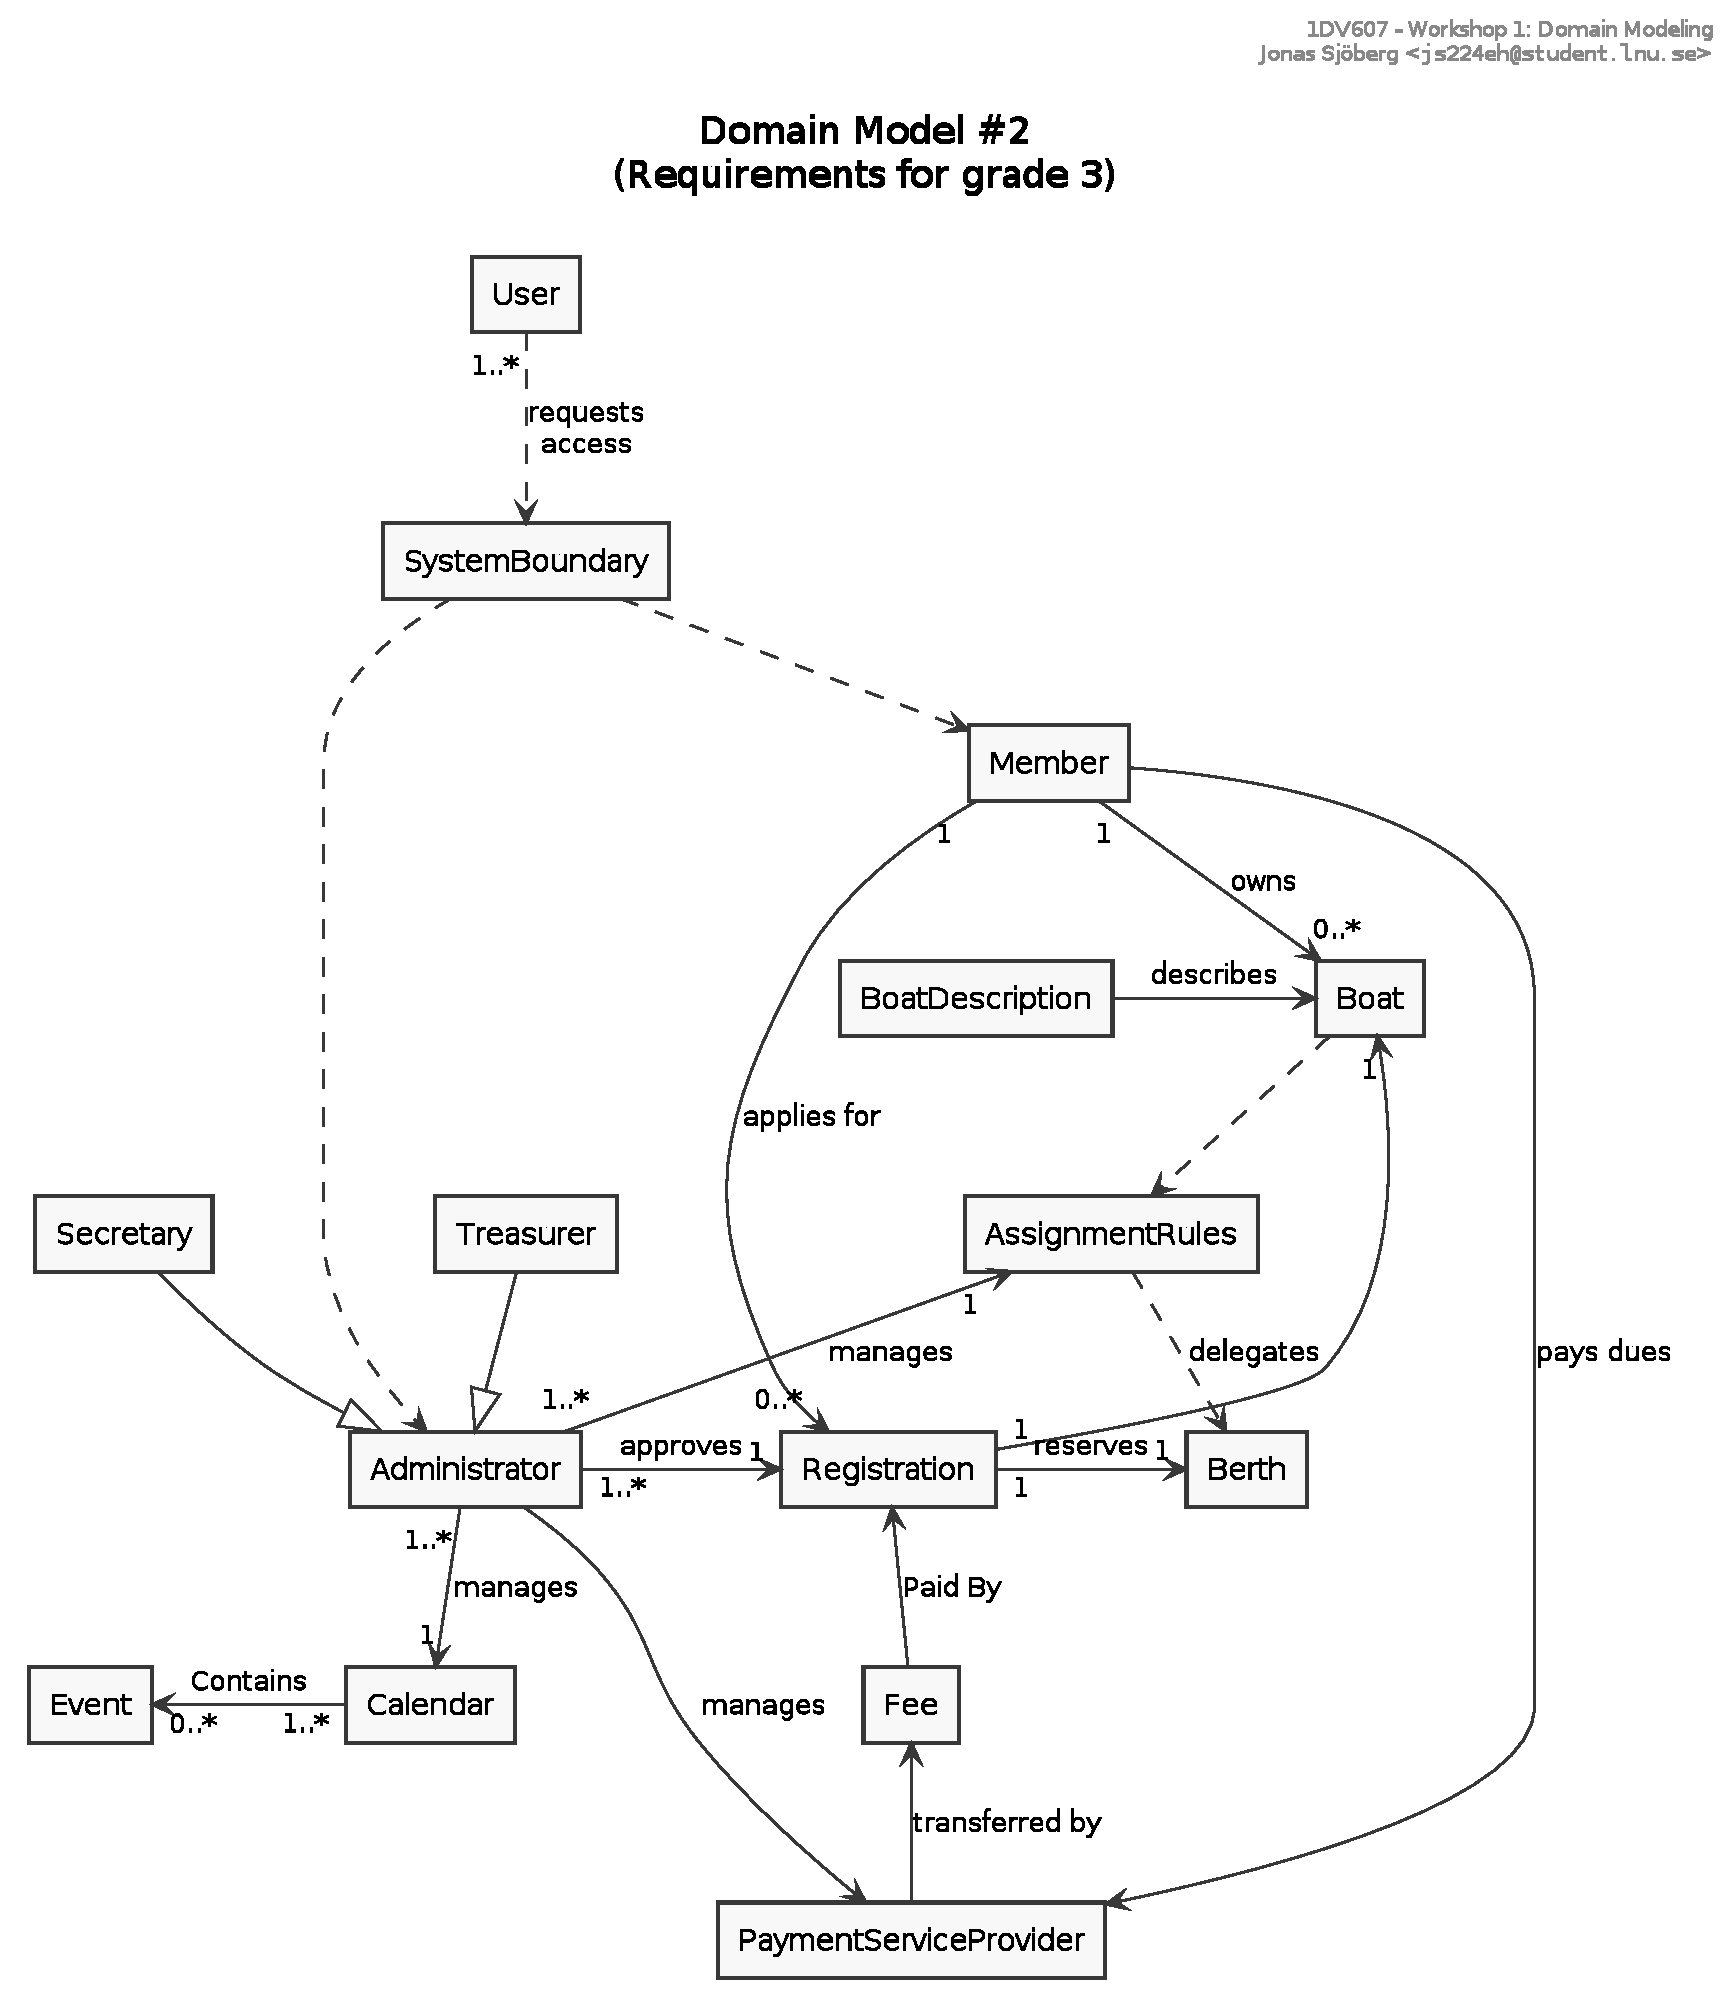
\includegraphics[width=\linewidth]{uml/domain-model_2.eps}
  \caption{UML Domain Model for Grade 3}
  \label{fig:uml-domain2}
\end{figure}

\subsubsection{Notes on the initial domain model}
The biggest change is the introduction of a payment service provider.

Most of the other requirements involve presentation of various data or managing
data in certain ways.  This is restricted to the different user-levels,
administrators should be able to manage invoices, etc.  These requirements
could be modeled with ``description classes'', which have been omitted for
clarity.


\subsection{Analysis of Requirements for Grade 4}
For this analysis, I've chosen to look at my open source project
``autonameow''\cite{js:autonameow-github}.  I've tried to model the system of
storage and retrieval of arbitrary data. However, this system is already
implemented and very complex --- the given model is incomplete and includes
many conflicting levels of abstraction.


\subsubsection{Notes on the main renaming actions in ``autonameow''}
The application collects as much data as possible from files. This includes the
file name, filesystem information, embedded metadata for various format,
textual contents, optical character recognition for images, etc. 

This data is then used to construct file names and rename files, using some
heuristics and user-control.

A highly simplified view of the main file remaing process is modeled in
Figure~\ref{fig:uml-domain3a}.


\subsubsection{Domain Model for Grade 3 -- file renaming in ``autonameow''}
\begin{figure}[htbp]
  \centering
  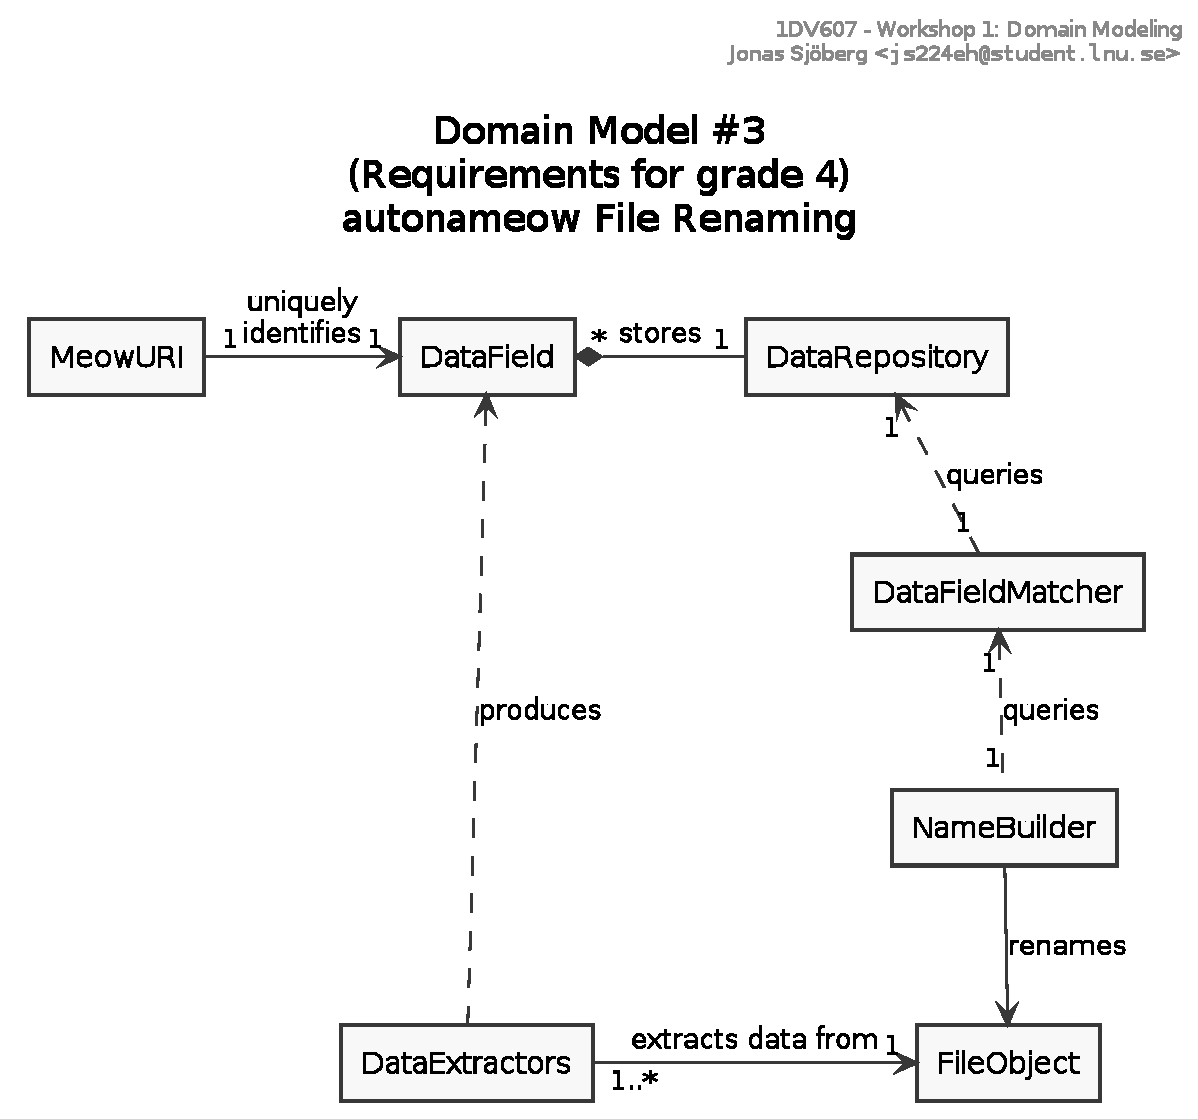
\includegraphics[width=\linewidth]{uml/domain-model_3a.eps}
  \caption{Domain Model of ``autonameow'' file renaming}
  \label{fig:uml-domain3a}
\end{figure}


\subsubsection{Notes on the ``autonameow'' data model}
Like a library or other storage system, stored data is given an identifier,
called a ``meowURI''; where ``URI'' is an abbreviation for Uniform Resource
Locator. These URIs provide the main means of querying and storing data.

A library might use ISBN- or EAN-numbers to identify specific items.
``autonameow'' also uses several identifiers, among these are ISBN-numbers,
which should be combined and weighted using some heuristics to produce a
suitable final result for any given query.
The user might want to include a creation date in the file name, the program
must then decide which of all the available date/time-information is most
likely ``correct''.


\subsubsection{Domain Model for Grade 3 -- data storage in ``autonameow''}
This model tries to capture the interaction between components. In practice, I
find that the interaction is too difficult to model properly at a level of
abstraction that would provide any additional insight, over what the source
code already provides.

A simplified model of the internal data storage is shown in
Figure~\ref{fig:uml-domain3b}.


\begin{figure}[htbp]
  \centering
  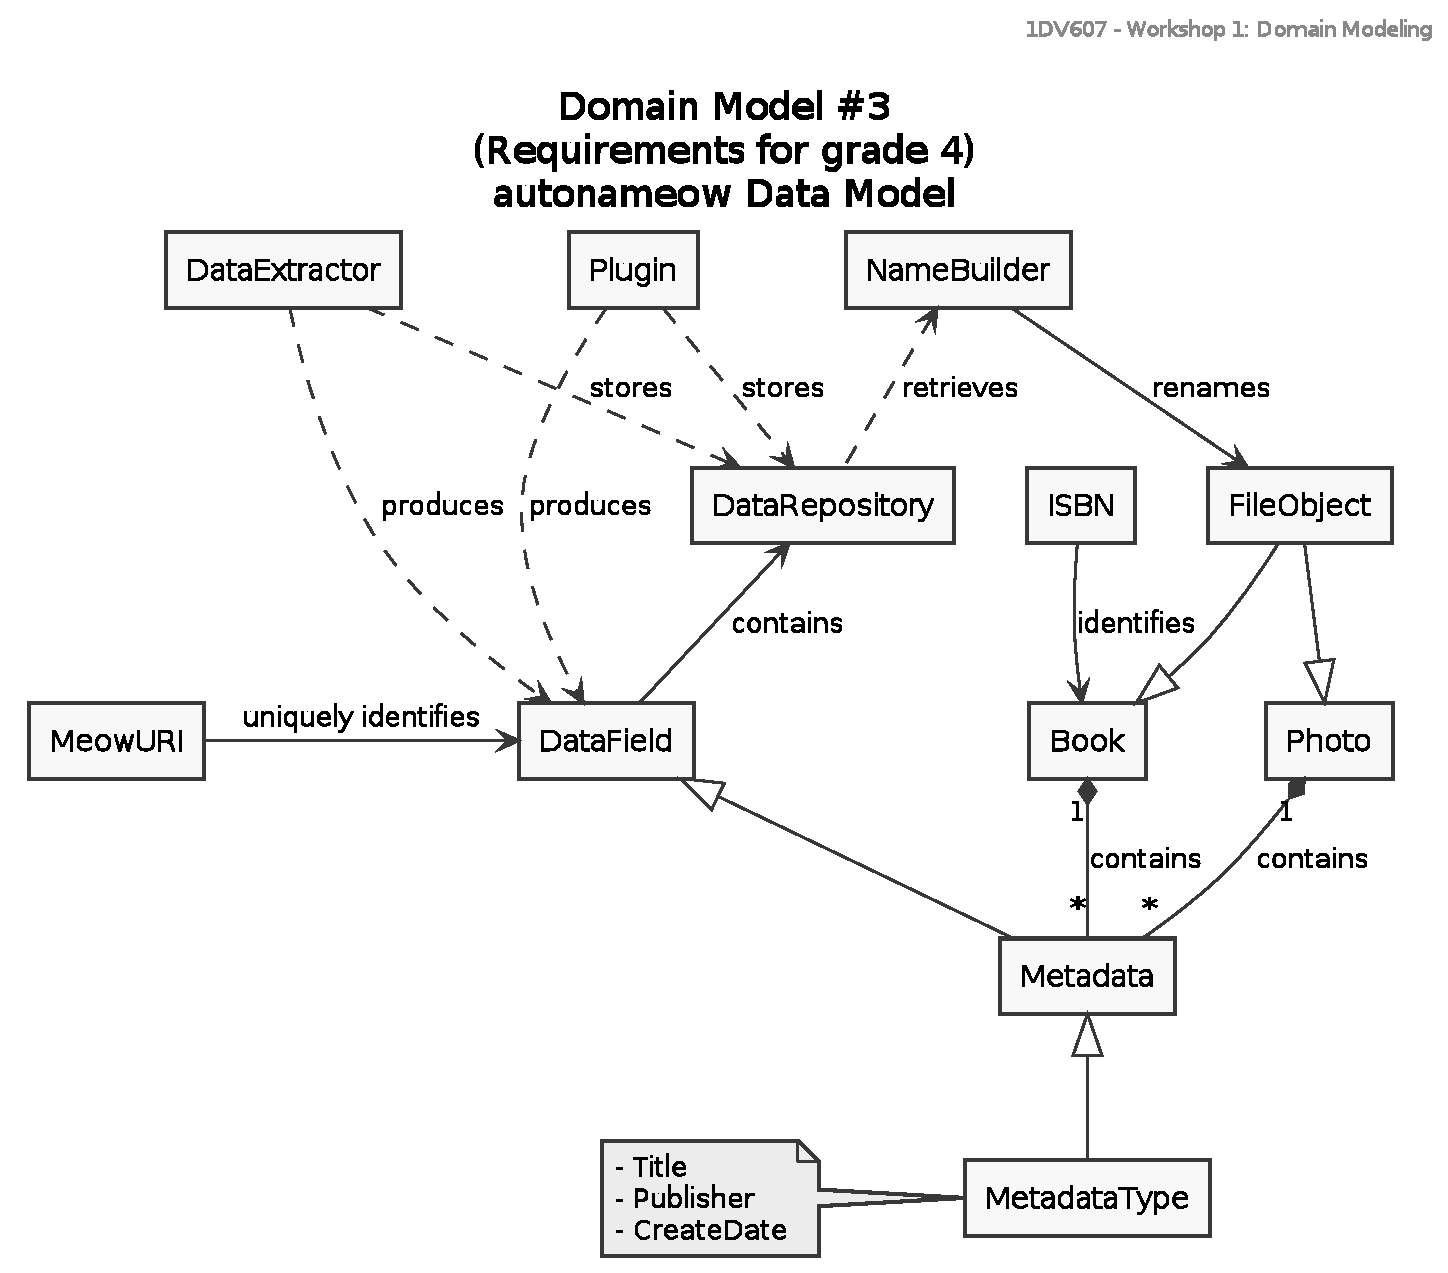
\includegraphics[width=\linewidth]{uml/domain-model_3b.eps}
  \caption{Domain Model of ``autonameow'' data storage}
  \label{fig:uml-domain3b}
\end{figure}

I've researched this topic for a very long time. A long list of references and
related projects or produces is included with the ``autonameow''
documentation\cite{js:autonameow-docs}.

Many models have proven incorrect or too complex. I will keep iterating and
redesigning the system until it meets the (ever changing) requirements.

I'm currently in the proces of redesigning the ``Repository'' to better handle
contextual information provided with a data item. Extracted metadata itself
often get additional metadata added on, containing the data source,
probabilities, primitive data types, etc \cite{metadata:aalemu-stevens}.
This has led me to research data repositories --- where methods of retrieval,
storage and presentation are all abstracted. I'm still reading up on how this
works.


  % ______________________________________________________________________________
%
%   1DV607 Objectorienterad Analysis och Design med UML
%   Workshop 1 --- "Domain Modeling"
%
%  Author:  Jonas Sjöberg
%           Linnaeus University
%           js224eh@student.lnu.se
%           https://github.com/jonasjberg
%
% License:  Creative Commons Attribution 4.0 International (CC BY 4.0)
%           <http://creativecommons.org/licenses/by/4.0/legalcode>
%           See LICENSE.md for additional licensing information.
% ______________________________________________________________________________


% ______________________________________________________________________________
\section{Conclusion}
%
% Conclusion - Here you will make you recommendation based on your analysis.
%
I have really struggled with understanding this very strange method of
designing software. Everything does not belong in a class. Orienting the
programming around objects, as in \emph{Object-Oriented} Programming; just
seems plain wrong and limiting.  This kind of UML-modeling and OO-design just
does not seem very useful when implementing systems in a procedural style, with
only a handlful of classes.

The abstract model often falls apart and become a tangled mess when attempting
to model the actually interesting parts, often ``cross-cutting concerns''. 

Most interesting problems and behaviours in non-trivial systems, where one
might benefit from modeling tools to aid in design and understanding --- are
cross-cutting.

Looking ahead, I will look at techniques to apply the object-oriented modeling
approach to my somewhat mixed (procedural, functional, object-oriented)
approach to thinking about programming, computing and complex systems.



  \addcontentsline{toc}{section}{References}
  \printbibliography{}

\end{document}
